%
%  =======================================================================
%  ····Y88b···d88P················888b·····d888·d8b·······················
%  ·····Y88b·d88P·················8888b···d8888·Y8P·······················
%  ······Y88o88P··················88888b·d88888···························
%  ·······Y888P··8888b···88888b···888Y88888P888·888·88888b·····d88b·······
%  ········888······"88b·888·"88b·888·Y888P·888·888·888·"88b·d88P"88b·····
%  ········888···d888888·888··888·888··Y8P··888·888·888··888·888··888·····
%  ········888··888··888·888··888·888···"···888·888·888··888·Y88b·888·····
%  ········888··"Y888888·888··888·888·······888·888·888··888··"Y88888·····
%  ·······························································888·····
%  ··························································Y8b·d88P·····
%  ···························································"Y88P"······
%  =======================================================================
% 
%  -----------------------------------------------------------------------
% Author       : 焱铭
% Date         : 2023-07-01 15:54:14 +0800
% LastEditTime : 2023-07-05 14:02:05 +0800
% FilePath     : \SCI-LaTeX-Submission-Process-for-Elsevier\EN-Manuscript.tex
% Description  : Manuscript-CN ⇒ Manuscript-CN ⇒ Major-Revision ⇒ Minor-Revision ⇒ Accepted Manuscript ⇒ Final Manuscript
%  -----------------------------------------------------------------------
%

\documentclass[preprint,5p,sort&compress,times,10pt]{elsarticle} % preprint review  % compress压缩引用序号 
%% Use the option review to obtain double line spacing
%% \documentclass[authoryear,preprint,review,12pt]{elsarticle}

%% Use the options 1p,twocolumn; 3p; 3p,twocolumn; 5p; or 5p,twocolumn
%% for a journal layout:
%% \documentclass[final,1p,times]{elsarticle}
%% \documentclass[final,1p,times,twocolumn]{elsarticle}
%% \documentclass[final,3p,times]{elsarticle}
%% \documentclass[final,3p,times,twocolumn]{elsarticle}
%% \documentclass[final,5p,times]{elsarticle}
%% \documentclass[final,5p,times,twocolumn]{elsarticle}

% ------------------------------------------------------------------------------------------------------------
%                                                  前言设置
% ------------------------------------------------------------------------------------------------------------
% 公式
\usepackage{amsmath} % 公式输入需要 equation 以及多行公式 [fleqn] 所有公式左对齐
\usepackage{amssymb} % The amsthm package provides extended theorem environments
\usepackage{xcolor} % 修稿标注时所需颜色宏
\usepackage{lineno} % 该宏包可显示行号


% % -----------------------------------------------------
% %                        中文高亮文本设置               *******************************************************
% % -----------------------------------------------------
% \usepackage{ctex} % 中文宏包,取消注释即可输入中文内容 
% \usepackage{xeCJKfntef} % 中文高亮设置,导入此包支持汉字特殊下划线效果 
% \newcommand{\gl}{\CJKsout*[thickness=2.5ex,format=\color{yellow}]} % 新定义高亮命令\gl 用来高亮显示中文

% -----------------------------------------------------
%                        表格格式设置
% -----------------------------------------------------
\usepackage[caption=false,farskip=0pt,labelfont={bf}]{subfig} % 设置子图所需宏包
\usepackage{booktabs} % 三线表
\usepackage{array} % 设置表格单元宽度
\usepackage{multirow} % 表格行合并单元格设置
\usepackage{threeparttable} % 添加表格注释

\usepackage[labelfont={bf}]{caption} % 题注字体加粗
\usepackage{setspace}  % 使用间距宏包

% -----------------------------------------------------
%                        术语表设置
% -----------------------------------------------------
\usepackage{ifthen}
\usepackage{framed} % Framing content
\usepackage{multicol} % Multiple columns environment
\usepackage[]{nomencl} % Nomenclature package %noprefix
\usepackage{etoolbox}

% 术语表详细设置
\renewcommand*\nompreamble{\begin{multicols}{2}} % 设置术语表为双栏显示
\renewcommand*\nompostamble{\end{multicols}}

% 更改术语之间的垂直行间距
\newlength{\nomitemorigsep}
\setlength{\nomitemorigsep}{\nomitemsep}
\setlength{\nomitemsep}{-1.25\parsep} % Baseline skip between items

% 创建术语表分组
\renewcommand{\nomgroup}[1]{%
\ifthenelse{\equal{#1}{A}}{\vspace{6pt} \item[\textbf{Greek symbols}]}{%
\ifthenelse{\equal{#1}{B}}{\vspace{6pt} \item[\textbf{Subscripts}]}{%
\ifthenelse{\equal{#1}{C}}{\vspace{6pt} \item[\textbf{Abbreviations}]}{}
}}

\itemsep\nomitemsep % 应用上面设置的术语垂直行间距
}
\makenomenclature % 打印术语表

% -----------------------------------------------------
%                        链接设置
% -----------------------------------------------------
\usepackage{hyperref} % 对目录生成链接,注:该宏包可能与其他宏包冲突,故放在所有引用的宏包之后
\hypersetup{colorlinks = true, % 将链接文字带颜色
    citecolor=blue, linkcolor=black, urlcolor=black,
	bookmarksopen = true, % 展开书签
	bookmarksnumbered = true, % 书签带章节编号
	pdftitle = Hydrothermal performance analysis of microchannel heat sink with embedded module with ribs and pin-fins, % 标题
	pdfauthor = Xue Bin Li} % 作者
    %\setlength{\mathindent}{0pt} % 将公式的缩进调整为0

% -----------------------------------------------------
%                        题注设置
% -----------------------------------------------------
\usepackage[capitalize]{cleveref} % 引用宏包 ,该宏包要在 hyperref后引用 noabbrev 引用前缀为缩写
% 关于题注的设置
\captionsetup[subfigure]{subrefformat=simple,labelformat=simple,listofformat=subsimple}
\renewcommand\thesubfigure{(\alph{subfigure})} % 该代码与上一行 设置引用前缀子图序号带圆括号
\renewcommand{\figurename}{Fig.} %题注中使默认的图名字改为图显示
\renewcommand{\tablename}{Table} %题注中使默认的表名字改为表显示
% \crefname{theorem}{定理}{定理}
% \crefname{lemma}{引理}{引理}
% \crefname{definition}{定义}{定义}
\crefname{figure}{Fig.}{Fig.} % 更改引用前缀 参数二为单独引用
\crefname{table}{Table}{Table} % 参数三为多个引用
\crefname{equation}{}{Eqs.}%Eq.
% \crefname{algorithm}{算法}{算法}

% -----------------------------------------------------
%                        自定义命令                     *******************************************************
% -----------------------------------------------------
\newcommand{\Process}{2-Manuscript-EN} % 根据投稿的进度修改该参数
\graphicspath{{\Process/Pictures/},}  % 图片所在文件夹,可放置多个文件夹,用,分隔。
\newcommand{\Nomenclature}{%
%  =======================================================================
%  ····Y88b···d88P················888b·····d888·d8b·······················
%  ·····Y88b·d88P·················8888b···d8888·Y8P·······················
%  ······Y88o88P··················88888b·d88888···························
%  ·······Y888P··8888b···88888b···888Y88888P888·888·88888b·····d88b·······
%  ········888······"88b·888·"88b·888·Y888P·888·888·888·"88b·d88P"88b·····
%  ········888···d888888·888··888·888··Y8P··888·888·888··888·888··888·····
%  ········888··888··888·888··888·888···"···888·888·888··888·Y88b·888·····
%  ········888··"Y888888·888··888·888·······888·888·888··888··"Y88888·····
%  ·······························································888·····
%  ··························································Y8b·d88P·····
%  ···························································"Y88P"······
%  =======================================================================
% 
%  -----------------------------------------------------------------------
% Author       : 焱铭
% Date         : 2023-07-04 21:34:35 +0800
% LastEditTime : 2023-07-04 21:43:54 +0800
% Github       : https://github.com/YanMing-lxb/
% FilePath     : \multi-objective_optimization_microchannel_heat_sink-with_embedded_module_with_ribs_and_pin-fins\Section\Nomenclature.tex
% Description  : 
%  -----------------------------------------------------------------------
%

\begin{table*}[!t]%!t % 该方法不适用于超过一页的符号说明

    \begin{framed}
        \begin{spacing}{1}
            \nomenclature[C,01]{LED}{light-emitting diod}
            \nomenclature[C,02]{LTCC}{Low temperature cofired ceramic}
            \nomenclature[C,03]{MATD}{mean absolute temperature deviation}
            \nomenclature[C,04]{MCHS}{microchannel heat sink}
            \nomenclature[C,05]{MCHS-SR}{straight rectangular microchannel}
            \nomenclature[C,06]{MCHS-REM}{microchannels with rib embedded module}
            \nomenclature[C,07]{MCHS-PFEM}{microchannels with pin-fin embedded module}
            \nomenclature[C,08]{MCHS-RPFEM}{microchannel heat sink with embedded module with rib and pin-fin}
            \nomenclature[]{$A$}{area on the chip's upper surface $(m^2)$}
            \nomenclature[]{$W_{rib}$}{width of the rib $(\mu m)$}
            \nomenclature[]{$H_{rib}$}{height of the rib $(\mu m)$}
            \nomenclature[]{$L_{rib}$}{length of the rib $(\mu m)$}
            \nomenclature[]{$d_{rib}$}{distance between the rib $(\mu m)$}
            \nomenclature[]{$S_{pf}$}{Side length of the pin-fin $(\mu m)$}
            \nomenclature[]{$H_{pf}$}{height of the pin-fin $(\mu m)$}
            \nomenclature[]{$Re$}{Reynolds number}
            \nomenclature[]{$N_{oc}$}{number of auxiliary channels}
            \nomenclature[]{$N_{mc}$}{number of main channels}



            \nomenclature[A]{$\rho_{f}$}{density of fluid $(kg/m^3)$}
            \nomenclature[A]{$\mu_{f}$}{dynamic viscosity of fluid $(kg/(m \cdot s))$}
            \nomenclature[A]{$\Lambda$}{molecule Knudsen number of water $(m)$}
            \nomenclature[A]{$\theta$}{MATD (Mean Absolute Temperature Deviation) $(K)$}
            \nomenclature[A]{$\alpha$}{Relative rib height}
            \nomenclature[A]{$\beta$}{Relative pin-fin height}
            \nomenclature[A]{$\gamma $}{Relative number of auxiliary channels}

            \nomenclature[B]{$s$}{solid}
            \nomenclature[B]{$f$}{fluid}
            \nomenclature[B]{$c$}{chip}
            \nomenclature[B]{$rib$}{rib}
            \nomenclature[B]{$pf$}{pin-fin}
            \nomenclature[B]{$ch$}{channel}
            \nomenclature[B]{$mc$}{main channels}
            \nomenclature[B]{$oc$}{auxiliary channels}

            \nomenclature[B]{$tot$}{total value}
            \nomenclature[B]{$ave$}{average value}
            \nomenclature[B]{$max$}{maximum value}

            \nomenclature[B]{$in$}{inlet}
            \nomenclature[B]{$env$}{environmental}

            \printnomenclature[23mm]

        \end{spacing}

    \end{framed}

\end{table*}} % 定义新命令\Nomenclature用于包含术语表的内容

% -----------------------------------------------------
%                        目标期刊
% -----------------------------------------------------
\journal{Applied Thermal Engineering} % 输入要投稿的期刊


% ------------------------------------------------------------------------------------------------------------
%                                                  正文内容
% ------------------------------------------------------------------------------------------------------------
\begin{document}
% \linenumbers % 增加行号 提交修改稿时用

% -----------------------------------------------------
%                        封面内容
% -----------------------------------------------------
\begin{frontmatter}


    \title{Hydrothermal performance analysis of microchannel heat sink with embedded module with ribs and pin-fins}

    \author[rvt]{Xuebin LI\corref{cor2}}
    \author[rvt]{Chunquan LI\corref{cor2}}
    \author[rvt]{Hongyan HUANG\corref{cor1}}%\fnref{fn1}
    \ead{hhy7844@guet.edu.cn}
    \author[rvt]{Yuanhao ZHENG}%\fnref{fn1}


    \cortext [cor1]{Corresponding author}  % 通讯作者
    \cortext [cor2]{These authors contributed to the work equllly and should be regarded as co-first authors.} % 共同一作声明,没有可去掉
    \fntext[fn1]{This is the specimen author footnote.} % 关于作者的介绍之类,没有可去掉

    \affiliation[rvt]{organization={Guilin University Of Electronic Technology}, %Department and Organization
        addressline={No.1 Jinji Road, Qixing District},
        city={Guilin},
        postcode={541004},
        state={the Guangxi Zhuang Autonomous Region},
        country={China}}

    \begin{abstract}
        A new microchannel heat sink with embedded modules with ribs and pin-fins is proposed as an effective solution to realize microchannel heat dissipation within low-temperature co-fired ceramic substrates.
    \end{abstract}

    % 图片摘要设置
    %Graphical abstract
    % \begin{graphicalabstract}
    %     \centering
    %     \includegraphics*[width=1 \textwidth]{Schematic.jpg}
    % \end{graphicalabstract}


    \begin{highlights}
        \item Microchannel cooling in a Low-Temperature Co-fired Ceramic substrate;
        \item A comparison with the performance of similar designs;
        \item Numerical study of three parameters of this microchannel heat sink.
    \end{highlights}

    \begin{keyword}
        Microchannel heat sink \sep Embedded modules \sep LTCC \sep Rib \sep Pin-fin
    \end{keyword}

\end{frontmatter}


%
%  =======================================================================
%  ····Y88b···d88P················888b·····d888·d8b·······················
%  ·····Y88b·d88P·················8888b···d8888·Y8P·······················
%  ······Y88o88P··················88888b·d88888···························
%  ·······Y888P··8888b···88888b···888Y88888P888·888·88888b·····d88b·······
%  ········888······"88b·888·"88b·888·Y888P·888·888·888·"88b·d88P"88b·····
%  ········888···d888888·888··888·888··Y8P··888·888·888··888·888··888·····
%  ········888··888··888·888··888·888···"···888·888·888··888·Y88b·888·····
%  ········888··"Y888888·888··888·888·······888·888·888··888··"Y88888·····
%  ·······························································888·····
%  ··························································Y8b·d88P·····
%  ···························································"Y88P"······
%  =======================================================================
% 
%  -----------------------------------------------------------------------
% Author       : 焱铭
% Date         : 2023-07-04 20:56:59 +0800
% LastEditTime : 2023-07-04 22:12:32 +0800
% FilePath     : \multi-objective_optimization_microchannel_heat_sink-with_embedded_module_with_ribs_and_pin-fins\Section\Section1.tex
% Description  : 
%  -----------------------------------------------------------------------
%

\section{Introduction}
\gl{散热重要性}

人工智能和第五代移动通信技术等系统技术的发展\cite{Lau_2022},推动着半导体行业在移动便携设备、高性能计算机、自动驾驶、物联网和大数据等应用领域的发展\cite{Lau_2022},同时也推动着电子芯片向着小型化和高集成化方向发展快速发展\cite{Sadique.Murtaza.ea_2022}。
在过去的几十年里处理器上的晶体管数量依照摩尔定律\cite{Tan.Du.ea_2021}的预测呈现出指数级的增长趋势,如这张50年间的微处理器的发展趋势图。
摩尔定律与登纳德定律\cite{liuyifan.zhangzhiyong_2022}引领着半导体行业飞速发展,半导体芯片上电子元件的数量与日俱增,大大提高了芯片的综合性能,但随着半导体芯片性能的提高,尺寸的限制,导致芯片工作时温度的急剧上升,这将对其正常的运行工作产生严重的影响。半导体芯片散热技术的发展已成为制约半导体芯片进一步发展的一大重要原因。


在先进制程方面,随着先进制程技术的飞速发展,推动着芯片的制程越来越接近物理极限,量子隧穿效应开始介入,使得晶体管的漏电现象出现,打破了登纳德定律使得晶体管在更小制程时静态功耗不减反增,产生了更多的热量。
芯片的散热问题成为了急需解决的问题。
与此同时,摩尔定律从 7 nm 工艺节点以后发展速度放缓,因此先进封装成为后摩尔时代的主力军\cite{WangRuoDa_2022}。
诸多学者提出了许多打破摩尔定律限制的技术,如2-D IC集成技术、2.1-D IC 集成技术\cite{Lau_2023,Chen.Lee.ea_2018,Huang.Hsu.ea_2018}、2.3-D IC集成技术\cite{Zhang.Gan.ea_2023,Lau.Chen.ea_2021}、2.5-D IC 集成技术\cite{Cai.Ma.ea_2018,BhuvanendranNairGourikutty.MengChow.ea_2020,Ding.Liu.ea_2020}和3-D IC集成技术\cite{Ding.Zhang.ea_2021,Huang.He.ea_2021,Marshall.Lee_2022}等。
这些高密度封装技术的发展使得微电子器件能够在有限的空间内叠加更多层的芯片以及集成更多的功能模块。
功能模块的高密度集成将会导致芯片在工作时发热量更大,使得整体系统的温度上升更大,严重影响芯片的正常工作。


电子设备失效的主要原因有:高温、潮湿、振动和灰尘\cite{He_2021}。
可以发现55\%的电子设备的失效是由于温度导致。
并在55\%的热失效中有很大一部分是由于温度分布的不均匀所导致。温度分布不均主要有两个原因:
一是工质沿着流道温度升高,热边界层变厚,传热系数降低,导致沿流道产生温度梯度,温度分布不均;
二是由于发热组件热通量分布不均而导致的温度分布不均。

电子器件散热方式主要分为两种\cite{QiWenLiang.ZhaoLiang.ea_2022},一是被动冷却如:自然对流散热\cite{ElGhandouri.ElMaakoul.ea_2020}、热电冷却\cite{DuanFeiFan.TuShuPing_2021}、热管冷却。二是主动冷却如:强迫风冷、液体对流散热\cite{Patil.Hotta_2022}、沸腾散热\cite{Markal.Kul.ea_2022,Markal.Kul_2022}、射流冲击散热\cite{LuJing.HuangLingLi.ea_2021,Li.Sun.ea_2023}、微通道散热\cite{Manda.Peles.ea_2021,Zhang.Wu.ea_2022,Ansari.Kim_2019,Ansari.Kim_2018,Soleymani.Rahimi.ea_2020}、喷雾散热\cite{Zhou.Feng.ea_2022}和相变储能冷却\cite{DuanFeiFan.TuShuPing_2021,WangYuanJin.ZhangSai.ea_2020,Kalbasi_2021}等。
在这些散热方式中风冷的散热能力较低,其散热极限仅为 $15\ \mathrm{W/cm^2}$,并且受到工作环境的限制,因此无法满足工作于特殊环境下的高热流密度集成电路的需求。
传统液体对流散热则是由于其体积过大,因此应用受到空间限制。
热电制冷则受制于热电材料的发展,尚未应用于高热流密度电子设备中。
而射流冲击与喷雾冷却结构复杂,对于空间的要求高,不适合于对芯片的散热。
相变储能冷却则具有时间迟滞性,相变材料具有不易封装的缺点,不适用于高热流密度的场景。
本文研究内容主要为针对于功率芯片进行散热,而微流道散热器具有结构紧凑、对流换热面积大、重量轻的优点,相对于上述的其他技术,微通道散热器实用性更强,更能满足研究内容的需求。


综上所述,当前半导体行业对散热技术发展有着迫切的需求。
先进制程技术的快速发展推动了芯片的小型化和高集成化,但同时也导致芯片工作时温度的急剧上升,影响了芯片正常运行。
高热流密度集成电路的发展也加剧了散热问题。
在传统的散热方式如风冷和液体对流散热等存在技术限制的情况下,微通道散热器应运而生,因其结构紧凑、对流换热面积大、重量轻等优点,更适用于高热流密度集成电路的散热需求。
但是,尽管微通道散热器具有更优的散热性能,但在某些情况下,比如LTCC基板中,仍然无法满足芯片高热流密度引起的散热需求。
因此,半导体行业仍需不断推动散热技术的发展,以满足不断增长的芯片散热需求。

本次研究提出的基于嵌入式散热模块的微通道散热技术,解决了工程项目中LTCC基板上由于芯片高热流密度所引起的散热问题,对集成电路、人工智能和第五代移动通信技术等应用领域的发展有着积极的意义。
该项技术具有散热性能高、温度均匀性好、可应用于多热源散热等优点,可有效增强芯片的散热性能,提高芯片的可靠性。
在半导体行业当前对芯片小型化和高集成化的需求下,该研究工作具有重要的实用意义和发展前景。
在此基础上作者通过一系列研究,提出了基于MC-RPF的多热源散热结构,并进行了优化设计和综合分析,为电子芯片散热问题的解决提供一种有效的技术方案和参考。

\Nomenclature




%
%  =======================================================================
%  ····Y88b···d88P················888b·····d888·d8b·······················
%  ·····Y88b·d88P·················8888b···d8888·Y8P·······················
%  ······Y88o88P··················88888b·d88888···························
%  ·······Y888P··8888b···88888b···888Y88888P888·888·88888b·····d88b·······
%  ········888······"88b·888·"88b·888·Y888P·888·888·888·"88b·d88P"88b·····
%  ········888···d888888·888··888·888··Y8P··888·888·888··888·888··888·····
%  ········888··888··888·888··888·888···"···888·888·888··888·Y88b·888·····
%  ········888··"Y888888·888··888·888·······888·888·888··888··"Y88888·····
%  ·······························································888·····
%  ··························································Y8b·d88P·····
%  ···························································"Y88P"······
%  =======================================================================
% 
%  -----------------------------------------------------------------------
% Author       : 焱铭
% Date         : 2023-07-04 20:57:38 +0800
% LastEditTime : 2023-07-04 21:44:56 +0800
% Github       : https://github.com/YanMing-lxb/
% FilePath     : \multi-objective_optimization_microchannel_heat_sink-with_embedded_module_with_ribs_and_pin-fins\Section\Section2.tex
% Description  : 
%  -----------------------------------------------------------------------
%

\section{Mathematical modeling of the microchannel heat sink}

\cref{fig:structure} shows the schematic design of MCHS-SR and the proposed MCHS-RPFEM.


\begin{figure*}[htbp] % figure* 可进行跨栏
    \centering % 居中
    \scriptsize % 设置字体
    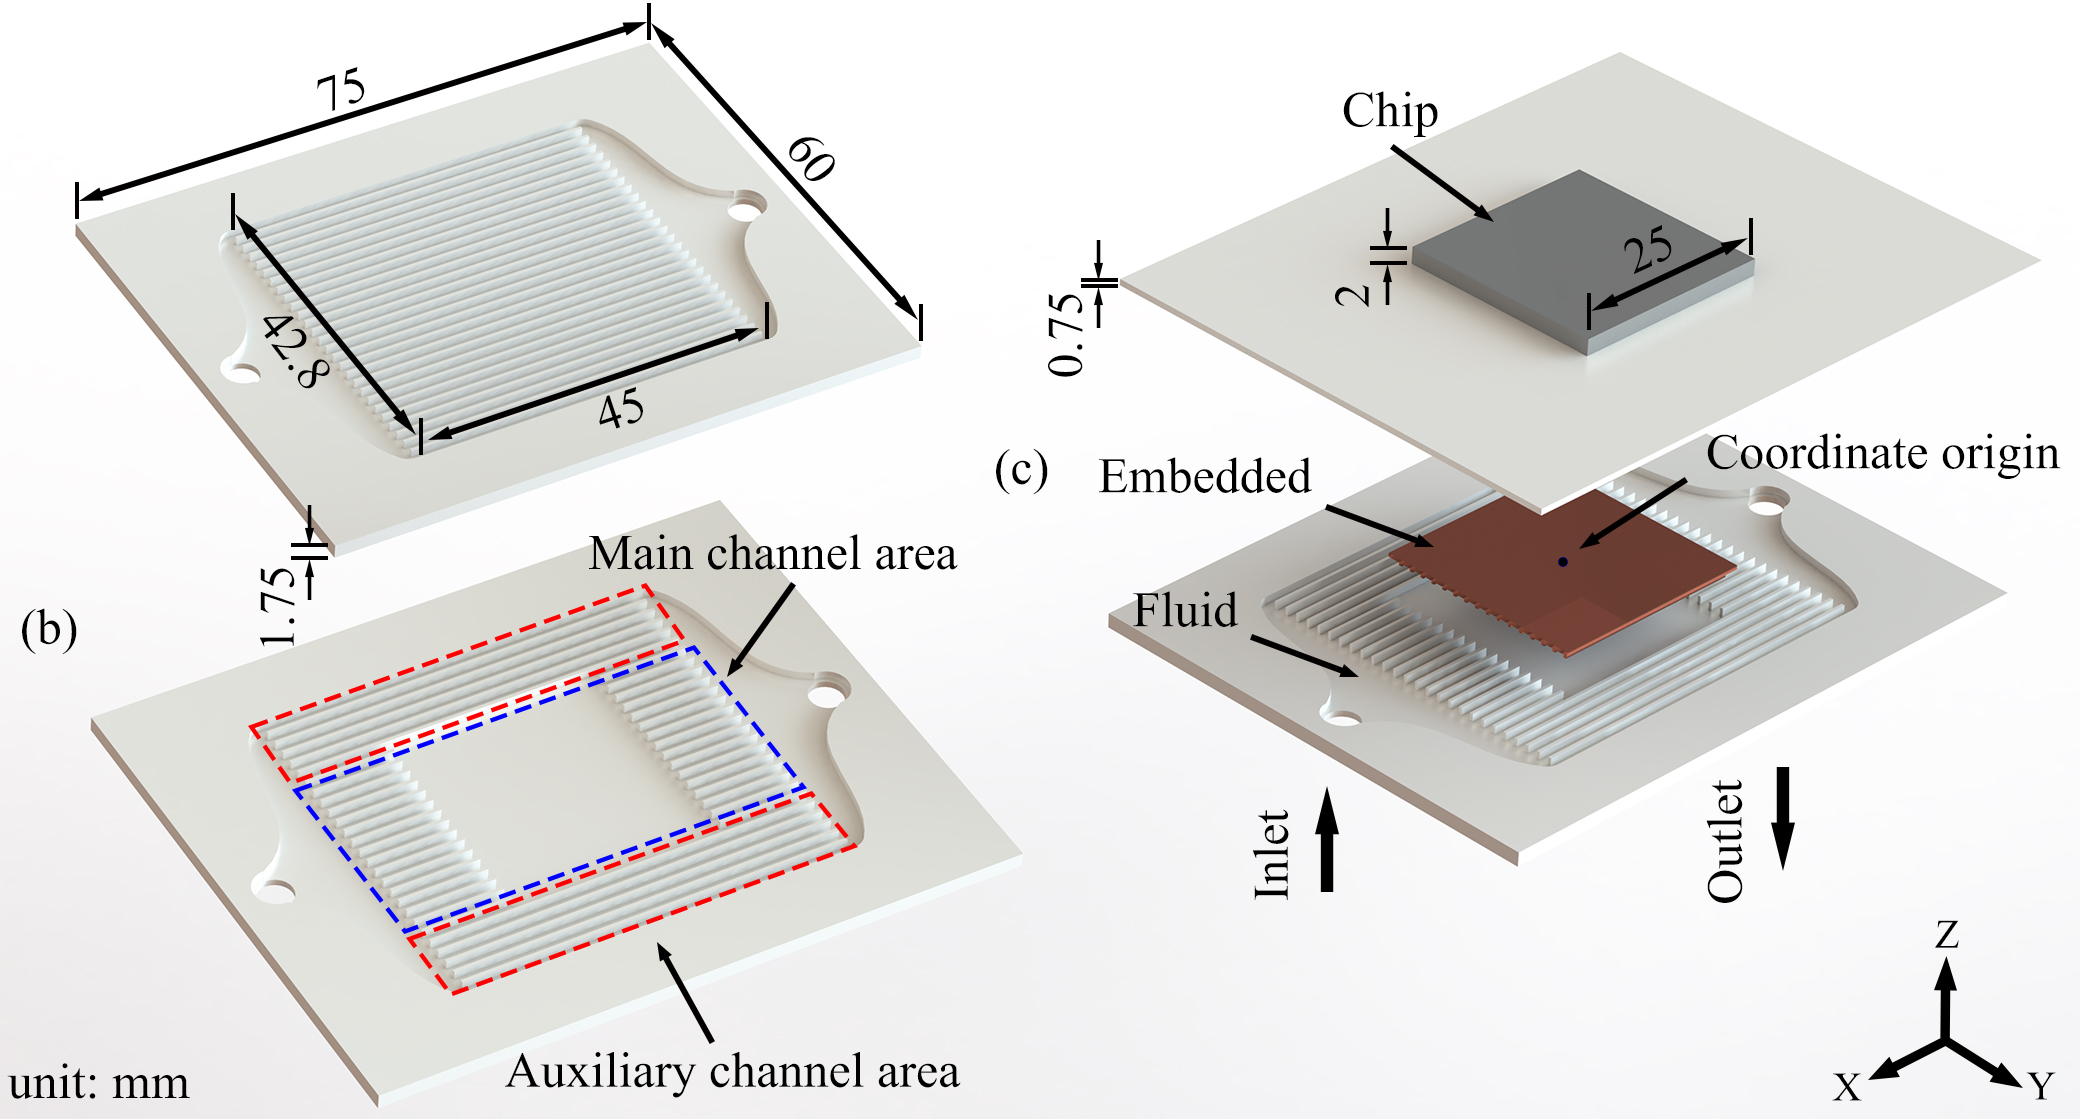
\includegraphics[width=1 \textwidth]{Schematic.jpg} % 
    \caption{
        (a) Straight rectangular microchannel (MCHS-SR),
        (b) microchannel heat sink with embedded modules with ribs and pin-fins (MCHS-RPFEM),
        (c) schematic diagram of the structure of MCHS-RPFEM.}
    \label{fig:structure}
\end{figure*}
Embedded module with ribs and pin-fins embedded in microchannel heat sink below chip.
\cref{tab:structure-parameter} shows the geometric parameters of the embedded module.
To investigate the effect of ribs and pin-fins on fluid flow and heat transfer on the embedded module in MCHS-RPFEM, three parameters were selected to be varied.
These three parameters are relative rib height ($\alpha$), relative pin-fin height ($\beta$), and relative number of auxiliary channels ($\gamma$).

\begin{table}[htbp]
    \centering
    \scriptsize
    \caption{MCHS-RPFEM geometric parameter table}
    \begin{tabular}{lccccccc}
        \toprule
        Geometrical parameters & $W_{rib}$ & $H_{rib}$ & $d_{rib}$ & $S_{pf}$ & $H_{pf}$ & $H_{ch}$ \\
        \midrule
        Value, $\mu m$         & 400       & 1000      & 1600      & 300      & 1000     & 1000     \\
        \bottomrule
    \end{tabular}
    \label{tab:structure-parameter}
\end{table}

%
%  =======================================================================
%  ····Y88b···d88P················888b·····d888·d8b·······················
%  ·····Y88b·d88P·················8888b···d8888·Y8P·······················
%  ······Y88o88P··················88888b·d88888···························
%  ·······Y888P··8888b···88888b···888Y88888P888·888·88888b·····d88b·······
%  ········888······"88b·888·"88b·888·Y888P·888·888·888·"88b·d88P"88b·····
%  ········888···d888888·888··888·888··Y8P··888·888·888··888·888··888·····
%  ········888··888··888·888··888·888···"···888·888·888··888·Y88b·888·····
%  ········888··"Y888888·888··888·888·······888·888·888··888··"Y88888·····
%  ·······························································888·····
%  ··························································Y8b·d88P·····
%  ···························································"Y88P"······
%  =======================================================================
% 
%  -----------------------------------------------------------------------
% Author       : 焱铭
% Date         : 2023-07-04 20:57:50 +0800
% LastEditTime : 2023-07-05 13:51:06 +0800
% Github       : https://github.com/YanMing-lxb/
% FilePath     : \SCI-LaTeX-Submission-Process-for-Elsevier\1-Manuscript-CN\Section\Section3.tex
% Description  : 
%  -----------------------------------------------------------------------
%

\section{Numerical method}

In this study, the following assumptions were made to simplify the numerical model: 

\begin{enumerate}[1.] % 可选类型 a) (i) Step 1.
    \item Newtonian fluid flow and steady laminar flow are used, and the fluid follows the Hagen-Poiseuille equation.
    \item The walls of the channel are rigid.
    \item Neglecting the effects of interaction forces, viscous heat, surface tension, and radiative heat transfer.
\end{enumerate}

\subsection{Governing equations and boundary conditions}

The governing equations are as follow:

Continuity equation:
\begin{equation}
    \nabla \cdot \left(\rho_f \vec{u}\right)=0
\end{equation}

Momentum equation:
\begin{equation}
    \vec{u} \cdot \nabla\left(\rho_f \vec{u}\right)=-\nabla p+\nabla \cdot\left(\mu_f \nabla \vec{u}\right)
\end{equation}

Energy equation for the fluid domain:
\begin{equation}
    \vec{u} \cdot \nabla\left(\rho_f C_{f} T_f\right)=\nabla \cdot\left(k_f \nabla T_f\right)
\end{equation}

Energy conservation equation for the solid domain:
\begin{equation}
    \nabla\left(k_s \nabla T_s\right)=0
\end{equation}
\textcolor{red}{}


The density ($\rho_{f}$), specific heat ($C_{f}$), thermal conductivity ($k_{f}$), and viscosity ($\mu_{f}$) of deionized water are correlated with the temperature as shown below:

\begin{figure*}[htb] % 将长公式放入figure* 环境中进行跨栏显示
    \begin{align}
        \rho_{f}(T)= & 999.9+9.561 \times 10^{-2} T-1.013 \times 10^{-2} T^{2}+8.459 \times 10^{-5} T^{3}-3.496 \times 10^{-7} T^{4}                      \\ \notag\\
        C_{f}(T)=    & 4217-3.452 T+1.155 \times 10^{-1} T^{2}-1.862 \times 10^{-3} T^{3}+1.538 \times10^{-5}T^{4}-4.850 \times 10^{-8} T^{5}             \\ \notag\\
        k_{f}(T)=    & 5.698 \times 10^{-1}+1.772 \times 10^{-3} T-4.870 \times 10^{-6} T^{2}-2.915 \times10^{-8} T^{3}+1.094 \times 10^{-10} T^{4}       \\ \notag\\
        \mu_{f}(T)=  & 1.750 \times 10^{-3}-5.558 \times 10^{-5} T+1.172 \times 10^{-6} T^{2}-1.579 \times10^{-8} T^{3}+1.169 \times 10^{-10} T^{4}\notag \\
                     & -3.535 \times 10^{-13} T^{5}
    \end{align}
\end{figure*}


where T is the temperature ($^{\circ}C$)


\subsection{Data reduction}


The performance of the four microchannel heat sinks was evaluated by their thermal resistance, Mean Absolute Temperature Deviation (MATD), and pressure drop.
Thermal resistance is defined as follows \cite{Ansari.Jeong_2021}:
\begin{equation}
    R_{th}=\frac{T_{c.max }-T_{in.max }}{Q_{tot}}
\end{equation}
$Q_{tot}$ is the chip's total heat produced, represented as:
\begin{equation}
    Q_{tot}=SV_{c}
\end{equation}

\subsection{Grid independence}

%
%  =======================================================================
%  ····Y88b···d88P················888b·····d888·d8b·······················
%  ·····Y88b·d88P·················8888b···d8888·Y8P·······················
%  ······Y88o88P··················88888b·d88888···························
%  ·······Y888P··8888b···88888b···888Y88888P888·888·88888b·····d88b·······
%  ········888······"88b·888·"88b·888·Y888P·888·888·888·"88b·d88P"88b·····
%  ········888···d888888·888··888·888··Y8P··888·888·888··888·888··888·····
%  ········888··888··888·888··888·888···"···888·888·888··888·Y88b·888·····
%  ········888··"Y888888·888··888·888·······888·888·888··888··"Y88888·····
%  ·······························································888·····
%  ··························································Y8b·d88P·····
%  ···························································"Y88P"······
%  =======================================================================
% 
%  -----------------------------------------------------------------------
% Author       : 焱铭
% Date         : 2023-07-04 21:20:55 +0800
% LastEditTime : 2023-07-05 13:40:59 +0800
% Github       : https://github.com/YanMing-lxb/
% FilePath     : \SCI-LaTeX-Submission-Process-for-Elsevier\2-Manuscript-EN\Section\Section4.tex
% Description  : 
%  -----------------------------------------------------------------------
%


\section{Results and discussion}

\subsection{Numerical validations}
To verify the accuracy of this simulation scheme, the numerical results are compared with the experimental data of several experiments \cite{Zhang.Wu.ea_2022,Qu.Mudawar_2002,Yang.Wang.ea_2017}, as shown in \cref{fig:Verification}.
\begin{figure*}[htbp]
    \centering
    \scriptsize% 设置字体大小
    \subfloat{
        \label{fig:Zhang}
        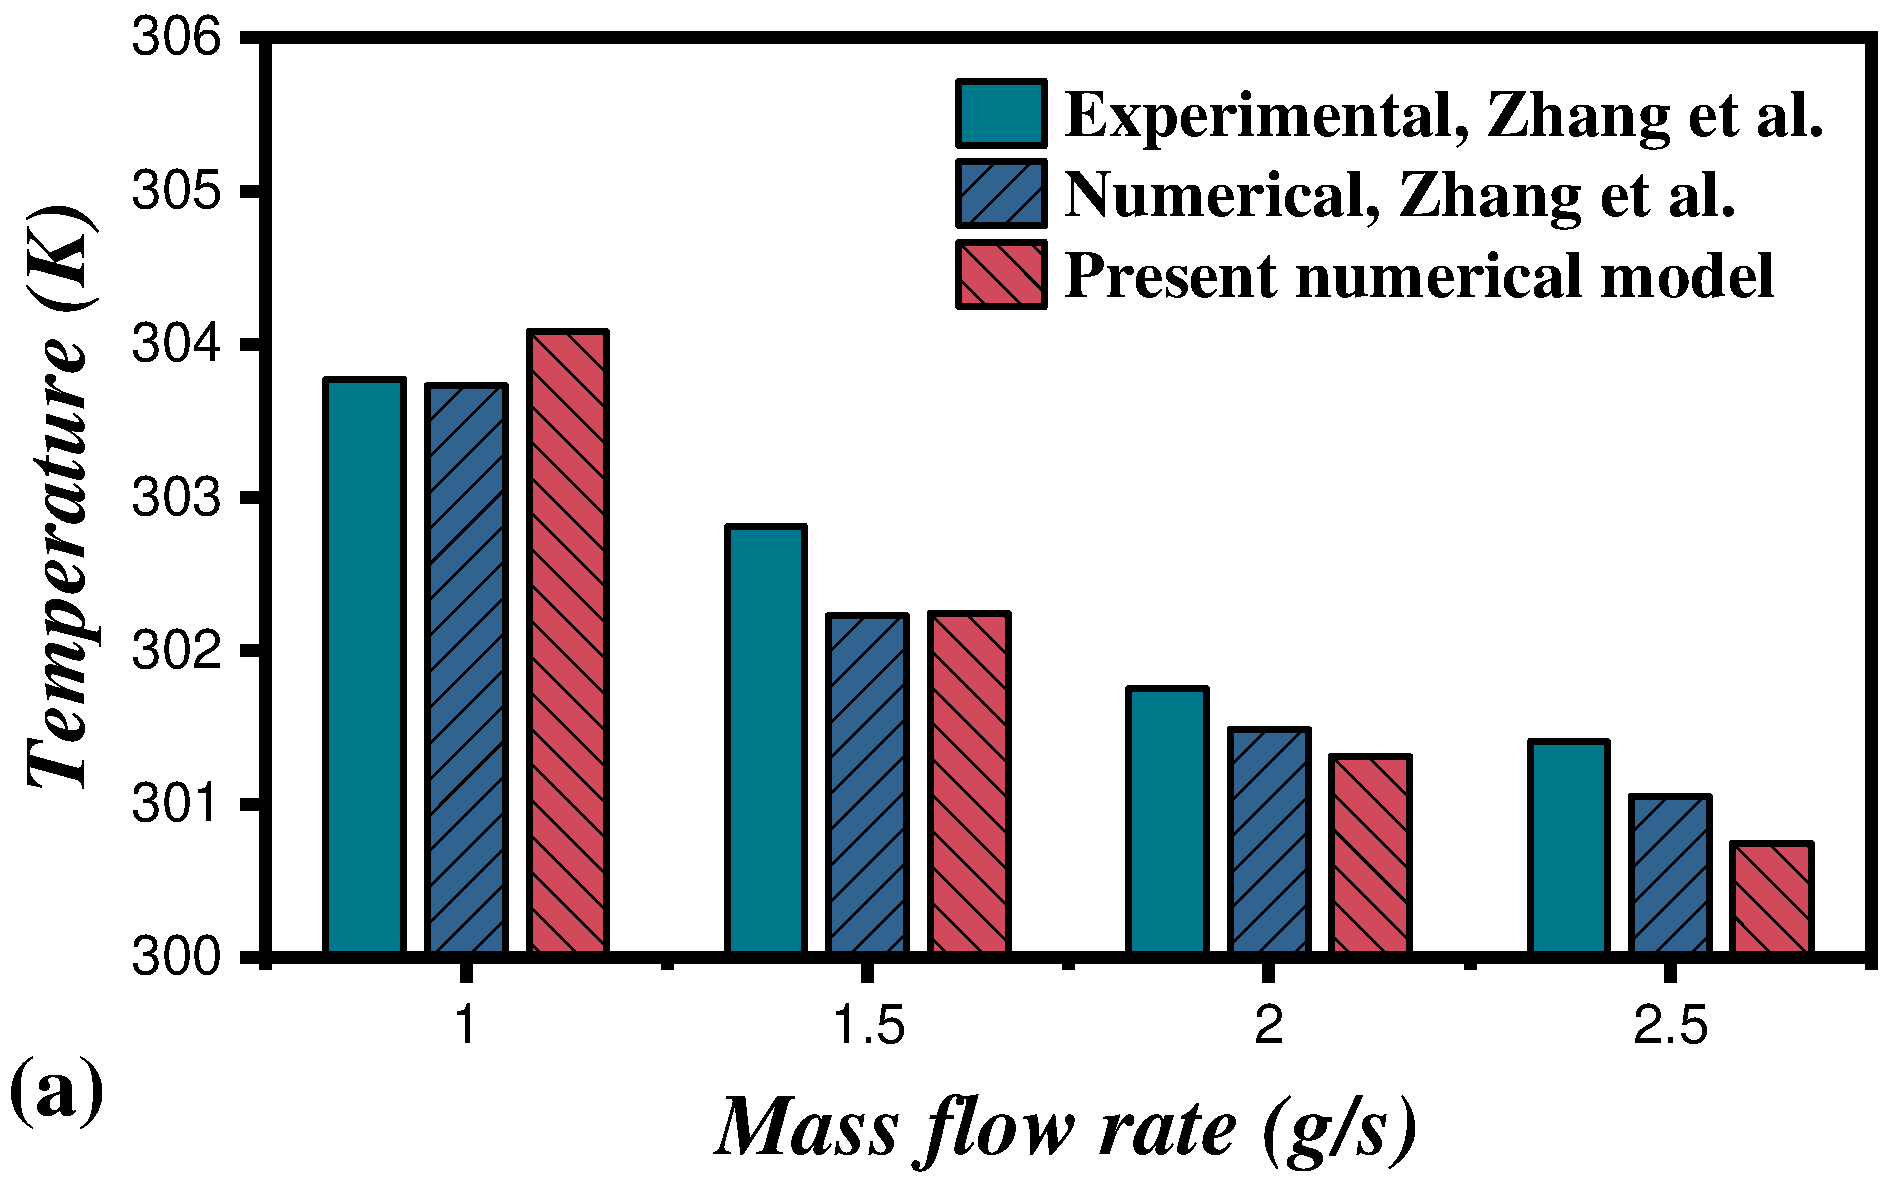
\includegraphics[width=0.35 \textwidth]{V-Zhang-T.pdf}} % 两个\subfloat之间加回车,图片会换行\hspace{2mm}
    \subfloat{
        \label{fig:Qu}
        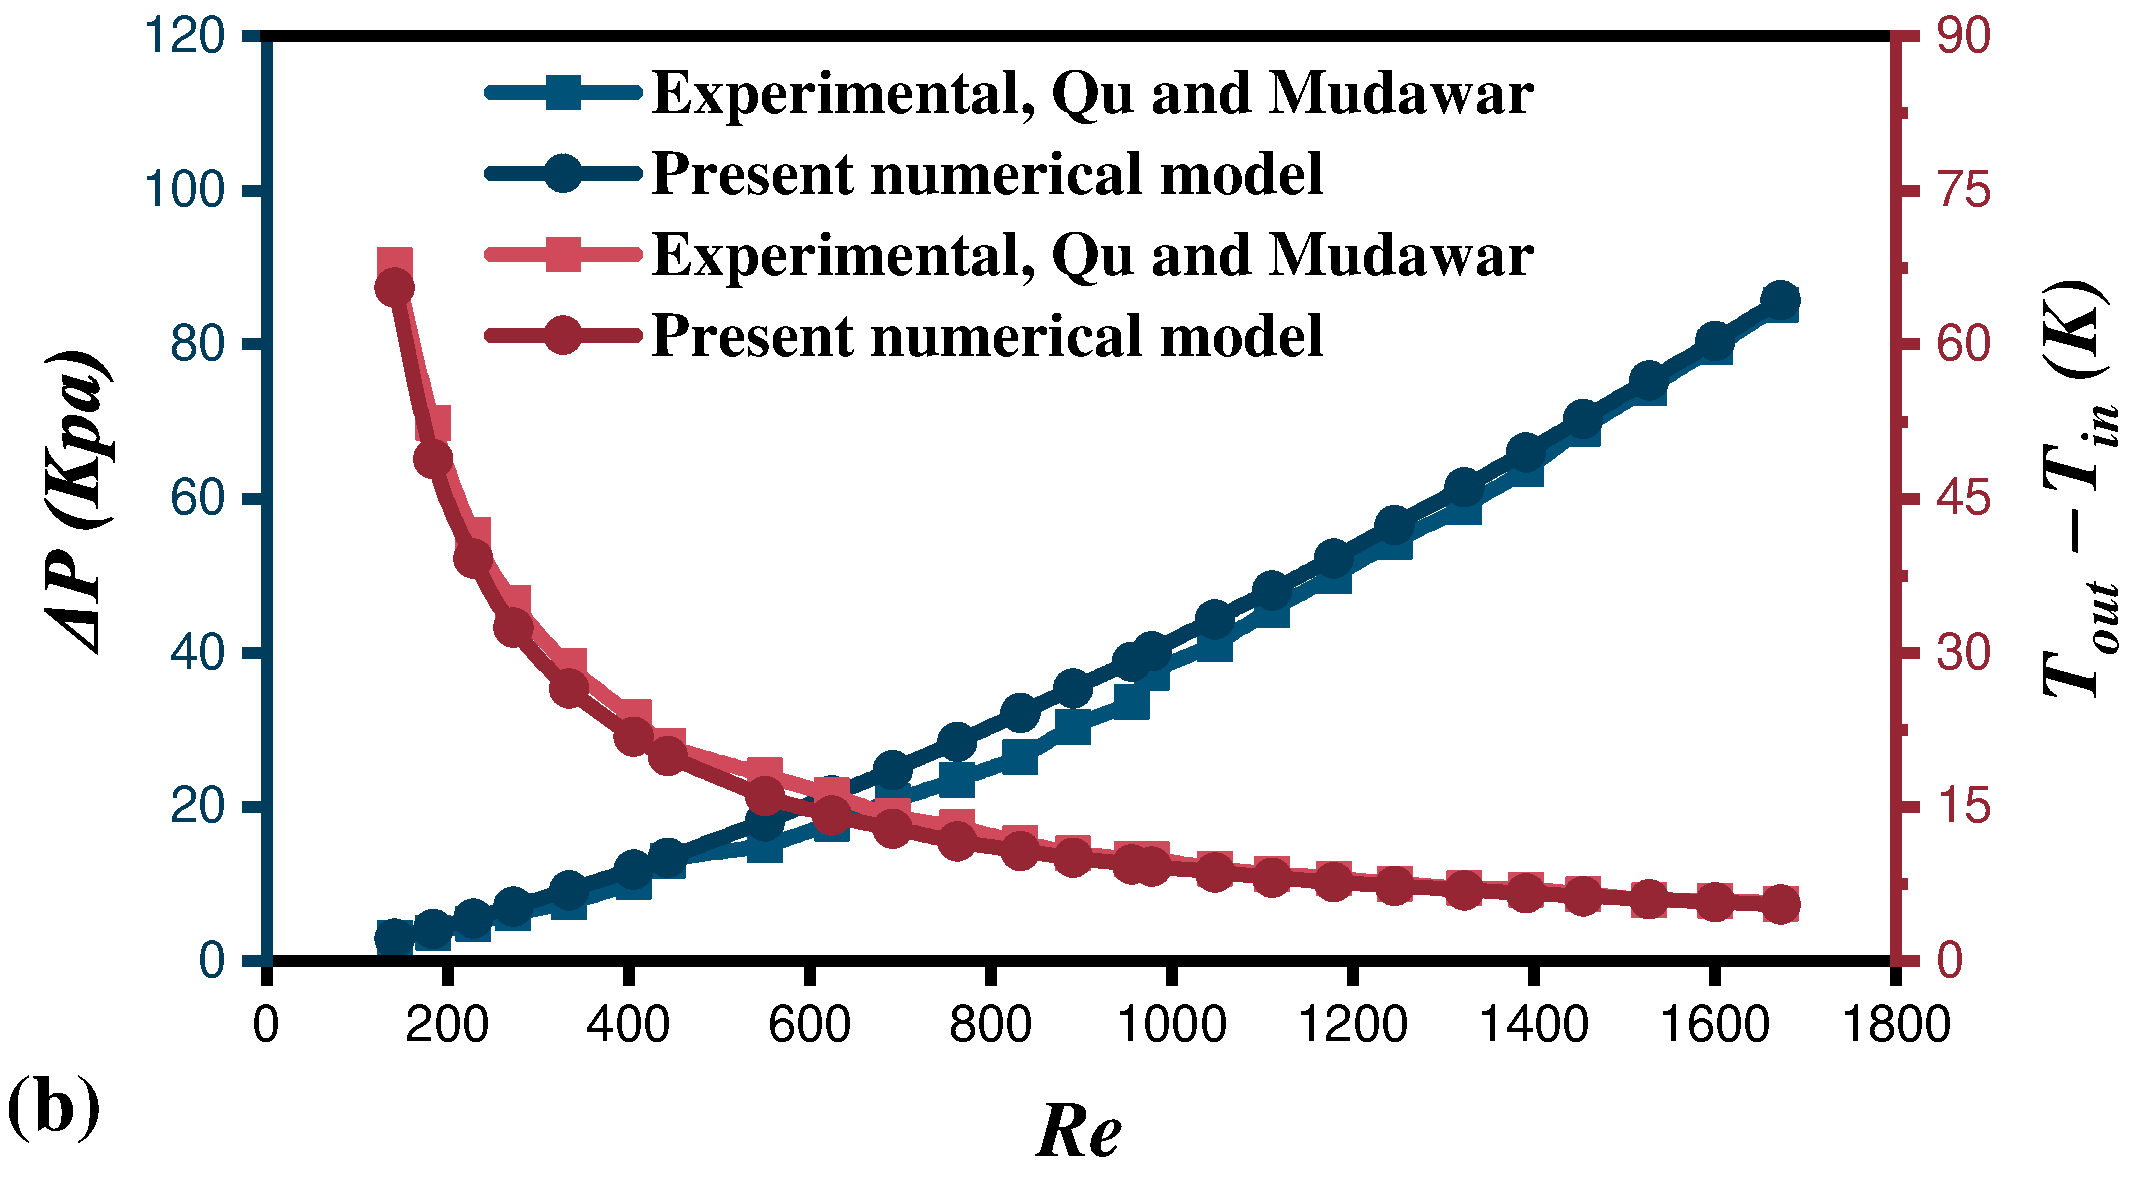
\includegraphics[width=0.4 \textwidth]{V-Qu-PT.pdf}}

    \subfloat{
        \label{fig:Yang}
        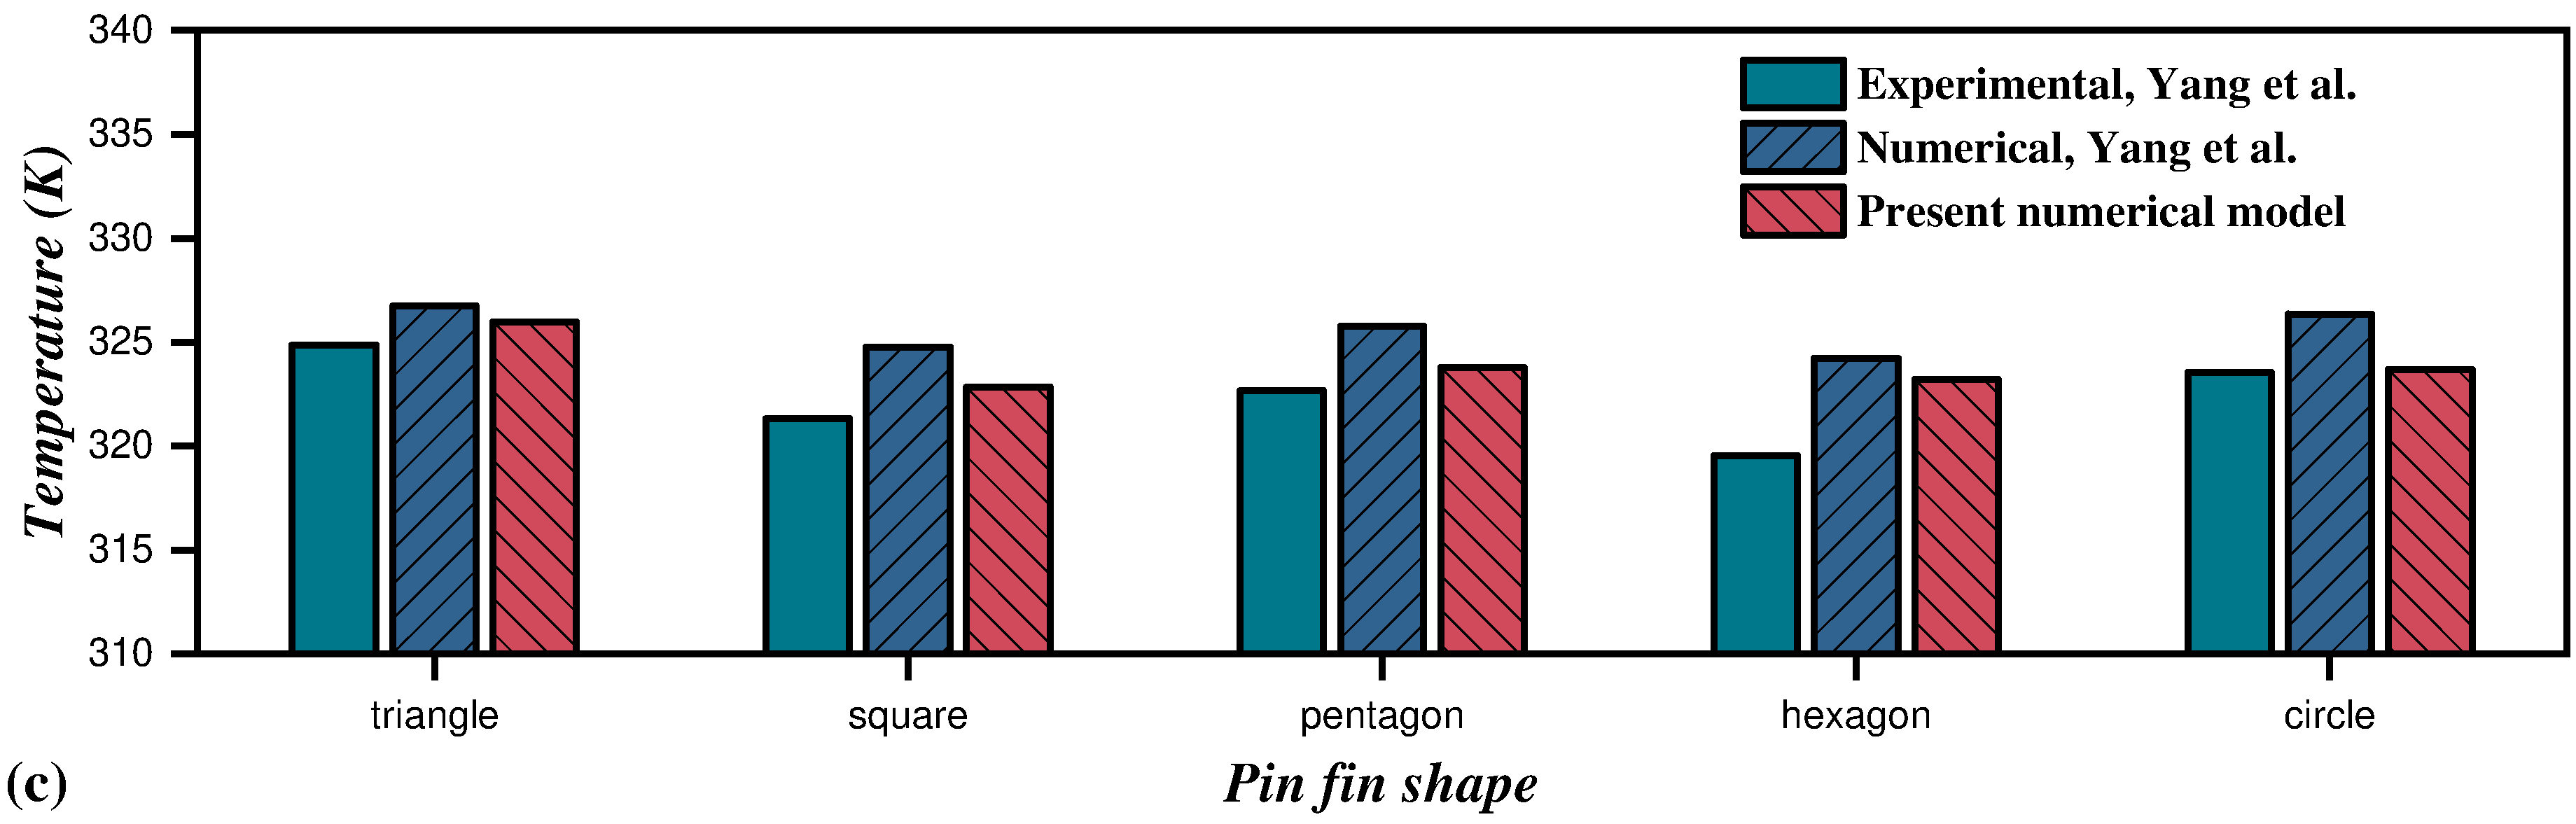
\includegraphics[width=0.75 \textwidth]{V-Yang-T.pdf}}
    \caption{Numerical validations.
        (a)Zhang et al. \cite{Zhang.Wu.ea_2022} of the microchannel heat sink at different mass flow rates for the variation of the bottom surface temperature of the microchannel heat sink.
        (b)Variation of inlet and outlet temperature difference and pressure drop in microchannels of Qu and Mudawar \cite{Qu.Mudawar_2002} at different Reynolds numbers.
        (c)Yang et al. \cite{Yang.Wang.ea_2017} of the pin-fin heat sink with the highest temperature on the bottom surface of the pin-fin heat sink for different pin-fin shapes.}
    \label{fig:Verification}
\end{figure*}

\subsection{Effect of geometric prameters on hydrothermal performance}

In order to explore the influence of the geometric




\subsubsection{The effect of relative rib height}

\subsubsection{Performance analysis}



\begin{table*}[!ht]
    \renewcommand{\arraystretch}{1.5} % 调整行距
    \centering
    \scriptsize
    \caption{Comparison with other solutions}
    \begin{threeparttable}
        \begin{tabular}{m{1.8cm}<{\raggedright}m{2.5cm}<{\raggedright}m{1.5cm}<{\raggedright}m{1.5cm}<{\raggedright}m{1cm}<{\raggedright}m{1.5cm}<{\raggedright}m{1.7cm}<{\raggedright}} \toprule
            Reference & Cooling methods & Heating area ($mm^2$) & Heat power ($W$) & Flow rate ($ml/min$) & Inlet pressure ($KPa$) & Maximum temperature ($^\circ C$) \\ \midrule
            \multirow{2}{*}{Zhang et al. \cite{Zhang.Zhang.ea_2015}} & \multirow{2}{2cm}{parallel cooling microchannels} & \multirow{2}{*}{$22\times 22$} & \multirow{2}{*}{75} & \multirow{2}{*}{58.1} & 330 & 99.52 \\ \cline{6-7}
            & & & & & $0.096^*$ & $55.7^*$ \\[5pt]
            \multirow{2}{*}{Yin et al. \cite{Yin.Li.ea_2019}} & \multirow{2}{2.2cm}{LTCC with embedded metal pillar arrays} & \multirow{2}{*}{$21\times 21$} & \multirow{2}{*}{20} & \multirow{2}{*}{18.85} & 7.12 & 74.85 \\ \cline{6-7}
            & & & & & $0.021^*$ & $57.35^*$ \\[5pt]
            \multirow{2}{*}{Liu et al. \cite{Liu.Jin.ea_2016}} & \multirow{2}{2.2cm}{LTCC with via holes and liquid metal} & \multirow{2}{*}{$10\times 10$} & \multirow{2}{*}{$30^{**}$} & \multirow{2}{*}{70} & \quad - & 83.85 \\ \cline{6-7}                                                                  
            & & & & & $0.138^*$ & $95.74^*$ \\[5pt]
            \multirow{2}{*}{Yu et al. \cite{YU.HAN.ea_2018}} & \multirow{2}{2.2cm}{LTCC with dual-layer spirals microchannels} & \multirow{2}{*}{$2\times 10$} & \multirow{2}{*}{$23^{**}$} & \multirow{2}{*}{45} & 370.7 & 84.85 \\ \cline{6-7}
            & & & & & $0.071^*$ & $55.54^*$\\\bottomrule
        \end{tabular}
        *\,\, The heat sink is MCHS-RPFEM and the coolant is deionized water.\\
        ** Heat flux($W/cm^2$)
    \end{threeparttable}
    \label{tab:Literature-comparison}
\end{table*}



%
%  =======================================================================
%  ····Y88b···d88P················888b·····d888·d8b·······················
%  ·····Y88b·d88P·················8888b···d8888·Y8P·······················
%  ······Y88o88P··················88888b·d88888···························
%  ·······Y888P··8888b···88888b···888Y88888P888·888·88888b·····d88b·······
%  ········888······"88b·888·"88b·888·Y888P·888·888·888·"88b·d88P"88b·····
%  ········888···d888888·888··888·888··Y8P··888·888·888··888·888··888·····
%  ········888··888··888·888··888·888···"···888·888·888··888·Y88b·888·····
%  ········888··"Y888888·888··888·888·······888·888·888··888··"Y88888·····
%  ·······························································888·····
%  ··························································Y8b·d88P·····
%  ···························································"Y88P"······
%  =======================================================================
% 
%  -----------------------------------------------------------------------
% Author       : 焱铭
% Date         : 2023-07-04 21:21:42 +0800
% LastEditTime : 2023-07-04 21:44:15 +0800
% Github       : https://github.com/YanMing-lxb/
% FilePath     : \multi-objective_optimization_microchannel_heat_sink-with_embedded_module_with_ribs_and_pin-fins\Section\Section5.tex
% Description  : 
%  -----------------------------------------------------------------------
%

\section{Conclusion}
To investigate the effect of



% section 加* 表示不显示序号
\section*{Declaration of Competing Interest}
The authors declare that they have no known competing financial interests or personal relationships that could have appeared to influence the work reported in this paper.
\section*{Formatting of funding sources}
This research did not receive any specific grant from funding agencies in the public, commercial, or not-for-profit sectors.

%% The Appendices part is started with the command \appendix;
%% appendix sections are then done as normal sections
%% \appendix

%% 参考文献
\bibliographystyle{elsarticle-num} % 加载参考文献样式文件
\bibliography{References} % 参考文献bib库

\end{document}
\endinput
%%
%% End of file `elsarticle-template-num.tex'.
